

\section{The ESMF Reference Manual for C}

ESMF has a complete set of Fortran interfaces and
some C interfaces.  This {\it ESMF Reference Manual} is a listing of 
ESMF interfaces for C.

Interfaces are grouped by class.  A class is comprised of the data and
methods for a specific concept like a physical field.  Superstructure classes 
are listed first in this {\it Manual}, followed by infrastructure 
classes.

The major classes in the ESMF superstructure are Components, which 
usually represent
large pieces of functionality such as atmosphere and ocean models,
and States, which are the data structures
used to transfer data between Components.  There are both data
structures and utilities in the ESMF 
infrastructure. Data structures include multi-dimensional Arrays, Fields
that are comprised of an Array and a Grid, and collections of Arrays
and Fields called ArrayBundles and FieldBundles, respectively.
There are utility libraries for data decomposition and communications,
time management, logging and error handling, and application configuration.

\begin{center}
\begin{figure}
\caption{Schematic of the ESMF ``sandwich'' architecture.
The framework consists of two parts, an upper level
{\bf superstructure} layer and a lower level {\bf infrastructure} layer.
User code is sandwiched between these two layers.}
\label{fig:TheESMFwich}
\scalebox{1.0}{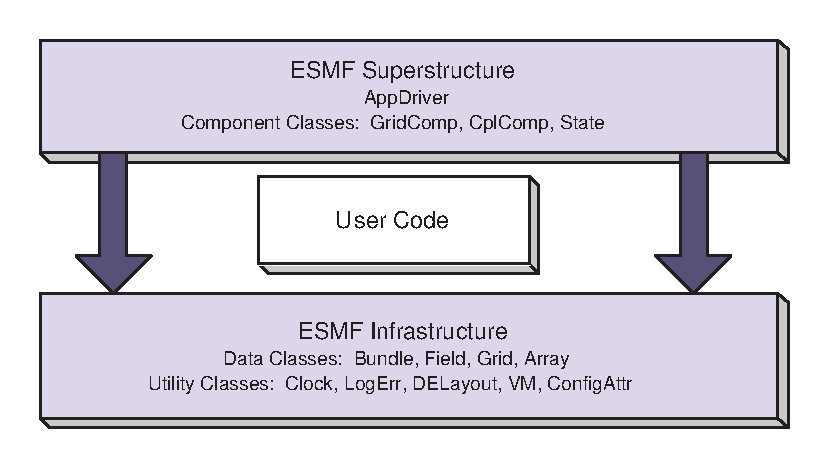
\includegraphics{ESMF_sandwich}}
\end{figure}
\end{center}

